\documentclass[10pt, a4paper]{article}
\usepackage[utf8]{inputenc}
\usepackage[T1]{fontenc,url}
\usepackage{multicol}
\usepackage{multirow}
\usepackage{parskip}
\usepackage{lmodern}
\usepackage{microtype}
\usepackage{verbatim}
\usepackage{amsmath, amssymb}
\usepackage{tikz}
\usepackage{physics}
\usepackage{mathtools}
\usepackage{algorithm}
\usepackage{algpseudocode}
\usepackage{listings}
\usepackage{enumerate}
\usepackage{graphicx}
\usepackage{float}
\usepackage{hyperref}
\usepackage{tabularx}
\usepackage{siunitx}
\usepackage{fancyvrb}
%\usepackage{natbib}
%\bibliographystyle{dinat}
\usepackage[makeroom]{cancel}
\usepackage[margin=2.0cm]{geometry}
\usepackage{pdfpages}
\usepackage[margin=10pt, textfont={small, it}, labelfont={bf}, labelsep=endash]{caption}
\renewcommand{\baselinestretch}{1}
\renewcommand{\exp}{e^}
\renewcommand{\b}{\boldsymbol}
\newcommand{\h}{\hat}
\newcommand{\m}{\mathbb}
\newcommand{\half}{\frac{1}{2}}
\renewcommand{\exp}{e^}
\renewcommand{\bar}{\overline}
\setlength\parindent{0pt}


\begin{document}
\title{AST5220\\ Exam 2020}
\author{
    \begin{tabular}{r l}
        Kandidatnummer & \texttt{15010}
    \end{tabular}}
% \date{}    % if commented out, the date is set to the current date

\maketitle

\section*{Problem 1 - Warm up}
\subsection*{a)}
Neutrinos decoupled earlier than photons from the thermal bath of the early cosmic plasma. During the period where photons were coupled, but neutrinos were not, the cosmic temperature fell to the order of the electron mass, at which point the electrons and positrons annihilated, releasing energy picked up by the photons but not the neutrinos.


\subsection*{b)}
A perfect fluid is a fluid which can be described solely by its pressure and density, and its equation of state is simply the ratio of the two:
\begin{equation}
    \omega = \frac{p}{\rho}
\end{equation}
The relative size of the universe relative to today is denoted $a$, and a value of $\ddot{a} > 0$ therefore describes a universe with accelerated expansion. The quantity $\ddot{a}$ is governed by the second Friedmann equation, which reads
\begin{equation}
    \frac{\ddot{a}}{a} = -\frac{4\pi G}{3}\qty(\rho + 3p) = - \frac{4\pi G}{3}\rho\qty(1 + 3\omega)
\end{equation}
With $a$ and $\rho$ both being non-negative, its clear that the equation of state which satisfies $\ddot{a} > 0$ is $\omega < -1/3$.


\subsection*{c)}
The CMB equations are a large set of coupled PDEs in real space, while in Fourier space they are separate ODEs for each $k$-mode, making solutions easier and more interpretable for each scale.


\subsection*{d)}
To detect a 1\% increase in the quadrupole we would obviously need an observational accuracy of comparable order. The margin of error for the small $\ell$ multipoles is very large due to a principle known as \textit{cosmic variance}. Cosmic variance is the inherit uncertainty in very large scale observations due to the physically limited sample size. For example, there are only a total of $m = 2\ell + 1 = 5$ quadrupoles to observe, resulting in a large uncertainty.


\subsection*{e)}
Calculating the multipoles $\Theta_\ell$ requires solving them all as a coupled set of ODEs, which might number in the thousands. Line of sight integration bypasses this by requiring only the first handful of $\ell$s, and calculation the rest from the \textit{source function}. The advantage is thus, as far as I know, purely in reduced computational complexity.


\subsection*{f)}
The visibility function is a probability distribution, defined as
\begin{equation}
    \tilde{g}(x) = -\dv{\tau}{x}\exp{-\tau}.
\end{equation}
It defines the probability that a photon performed a last scattering event as a time $x$. In other words, if you look out into the void of space, and a photon hits your eyes, the visibility function tells you the probability distribution of when the photon last encountered another particle.

The optical depth was incredibly high before recombination, meaning photons scattered a lot. This means that the probability of a photon last scattering any considerable amount of time before recombination is practically zero.


\subsection*{g)}
Both terms are first order perturbation, making it a second order term. In linear perturbation theory, we neglect second order terms. We could solve it from the geodesic equation. 


% \bibliography{ref}
% \bibliographystyle{plain}




\section*{Problem 2: The CMB and matter power-spectrum}
\subsection*{a)}
\subsubsection*{The Sachs-Wolfe effect}
\begin{equation}
    g(\Theta_0 + \Psi)
\end{equation}
The first term in the integrad is the Sache-Wolfe effect, which is the contribution from the local monopole at recombination to the anisotropies. The inclution of the visibility function demonstrates that the effect traces last scattering (as $g$ is virtually zero elsewhere), and that we observe a snapshot frozen in time of the last scattering monopole. In addition, the gravitational $\Psi$ term represents the effect of the photons having to climb out of the potential wells traced by $\Psi$.


\subsubsection*{The integrated Sachs-Wolfe effect}
\begin{equation}
    \qty(\dv{\Psi}{\eta} - \dv{\Phi}{\eta})\exp{-\tau}
\end{equation}
The second term is the integrated Sachs-Wolfe effect, which is the interaction of photons with changing gravitational potentials. As photons move through over and under-densities in an expanding universe, it might leave those regions with more or less energy than it entered with, due to their changing nature.

As we can see, the effect is mostly relevant at later times, as it contains an exponential suppression in $\tau$. In addition, it is only relevant when the gravitational potentials change rapidly, an effect seen for large scale anisotropies entering dark energy domination.


\subsubsection*{The Doppler term}
\begin{equation}
    -\frac{1}{k}\dv{(g v_b)}{\eta}
\end{equation}
The last term is known as the Doppler term, the reason for which is lost on me. It contains the effect from the strong coupling the photons have to baryons at last scattering (as we can see from the the inclusion of $g$, making it zero elsewhere.)


\subsection*{b)}
The Sachs-Wolfe plateau is caused by the late integrated Sachs-Wolfe effect, which amplifies large-scale anisotropies as the universe enters the dark energy dominated era. The gravitational potentials undergo a rapid decline as we enter this era (as we saw in milestone 3). The larger scales (small $\ell$) are much more affected, as they have much larger gravitational potentials to begin with, due to not being suppressed by the Meszaros effect in the early universe. This rapid fall in potentials again tilt the power-spectrum, through the Sachs-Wolfe term in the line of sight equation.

Several parameters, like the spectral index $n_s$, as well as the relative energy densities for dark energy and curvature $\Omega_\Lambda$ and $\Omega_k$, tilt the low-$\ell$ end of the power-spectrum in such a way. Neither are however completely degenerate with the late integrated Sache-Wolfe effect, as they all affect the high-$\ell$ end of the power spectrum as well.


\subsection*{c)}
Increasing the optical depth $\tau$ lowers the peaks and high-$\ell$ end of the temperature power-spectrum. A more optically thick reionization naturally washes out small-scale features in the CMB, as more scattering occurs.

Increasing $\tau$ leads to the same washing out of high-$\ell$ features in the polarization power spectrum. It does, however, majorly increase the E-mode polarization of the very largest scales. I know that Thomson scattering under a local quadropole leads to E-modes, although I don't know where a local quadropole would come from.

Increasing $\tau$ should have little or no impact on the matter power spectrum, as it is not probed by photon temperature, and usually measured by probing matter at low redshift.

Tau is somewhat degenerate with the spectral index $n_s$, but they can also be differentiated by their effect on the low-$\ell$ end of the temperature power spectrum, and their effect on the matter power spectrum (which $n_s$ affects).


\subsection*{d)}
This is a dampened harmonic oscillator, the first and third term being the familiar terms of an harmonic oscillator, and the second first order derivative in $h$ being a dampening term. The dampening does in this case come from the expansion of the universe, which dampens tensor perturbations over time. The damping is strongest for large $k$, meaning small tensor perturbations experience an exponential decay in the early universe.

The large scale (small $\ell$) perturbations, which are the only ones who survive until after recombination, have not yet entered the horizon when recombination happens. They are therefore not able to influence the CMB temperature perturbations.



\subsection*{e)}
$\Delta_m(x,k)$, being the gauge-invariant matter perturbation, grows as $\propto a^2$ at very early times, while the universe is radiation-dominated, and the perturbation is larger than the particle horizon. Also, as the perturbations enters the matter-dominated regime, they always grow as $\propto a$. However, perturbations which enter the particle horizon before having entered the matter-dominated era, undergo a era of suppressed growth of $\propto \log{a}$, until they finally enter matter-domination. This suppression is known as the Meszaros effect, and only affects perturbations below a certain scale. This scale is the $k_{peak}$ for which the power-spectrum peaks.

Calculating this peak is simply a matter of calculating the size of the particle horizon at the time of radiation-matter equality. The peak happens when the matter and radiation densities are equal, at
\begin{equation}
    \Omega_{m,0}a^{-3} = \Omega_{r,0}a^{-4} \quad\Rightarrow\quad a_{peak} = \frac{\Omega_{r,0}}{\Omega_{m,0}}
\end{equation}


A good approximation to the horizon scale is $c/\mathcal{H}$, giving an approximate k-peak at
\begin{align}
    k_{peak} &= \frac{a_{peak}H(a_{peak})}{c} = \frac{\Omega_{r,0} H_0\sqrt{\Omega_{r,0}a^{-4} + \Omega_{m,0}a^{-3}}}{c\Omega_{m,0}}\\
    &= \frac{\Omega_{r,0}H_0\sqrt{\Omega_{m,0}^4/\Omega_{r,0}^3 + \Omega_{m,0}^4/\Omega_{r,0}^3}}{c\Omega_{m,0}} = \frac{\sqrt{2}\Omega_{m,0}}{\sqrt{\Omega_{r,0}}}\frac{\SI{100}{h\cdot (km/s)/Mpc}}{c}
\end{align}
which, inserting for $\Omega_{r,0} \approx 5\times 10^{-5}$ and $\Omega_{m,0} \approx 0.3$ gives
\begin{equation}
    k_{peak} \approx \SI{0.04}{Mpc^{-1}}
\end{equation}

As we see from the expression for $k_{peak}$, there is a degeneracy between $h$, $\Omega_{m,0}$, and $\Omega_{r,0}$ as to the peak of the matter power spectrum.




\section*{Problem 3: Scattering processes involving baryons}

\begin{equation}
    \delta_{b}^{\prime}=\frac{c k}{\mathcal{H}} v_{b}-3 \Phi^{\prime}
\end{equation}

\begin{equation}
    v_{b}^{\prime}=-v_{b}-\frac{c k}{\mathcal{H}} \Psi+\tau^{\prime} R\left(3 \Theta_{1}+v_{b}\right)
\end{equation}


1. $p^{+} \gamma \rightarrow p^{+} \gamma$\\
Scattering of photons and protons do technically happen, but the cross section is very small (meaning its exceedingly unlikely to happen), so we can safely ignore this interaction in the collision term.

2. $e^{-} \gamma \rightarrow e^{-} \gamma$\\
Although very similar to the process we ignored above, the cross section of a electron-photon scatter is much larger due to the much lower mass of the electron, and this interaction is important to include in the collision term.

3. $e^{-} e^{-} \rightarrow e^{-} e^{-}$\\
The LHS of our Boltzmann equation contains the change in the baryons distribution function, e.g. their position and momentum. I believe that the symmetric nature of an elastic collision like this leaves the distribution function unchanged, making the interaction unimportant to the collision term.

4. $e^{-} e^{+} \leftrightarrow \gamma \gamma$\\
The annihilation of an electron and a positron to two photons, and the spontaneous decay of two photons into an electron and a position are both important interactions which impacts the number of baryons, and should therefore be included. However, only the former of these interactions happen spontaneously, and the latter requires a very high temperature to happen, which is only present in the very early universe. After this point, there will be no large abundance of positrons, and the former process becomes unimportant as well. In other words, this term quickly becomes unimportant after the universe cools.

5. $e^{-} p^{+} \rightarrow e^{-} p^{+}$\\
While this interaction should in theory be considered, it ends up not contributing to the distribution, due to symmetry.


6. $n \rightarrow e^{-} p^{+} \bar{\nu}_{e}$\\
This interactions drastically changes the distribution of baryons, but the timescale for free neutron decay is minutes, and protons and neutrons couple before that, making this interaction unimportant.


7. $e^{-} \nu_{e} \rightarrow e^{-} \nu_{e}$\\
As number 5, this could change the momentum distribution of the baryons, but neutrinos also decouple very early, making this term less important.


\section*{Problem 4: Recombination including Helium}
\subsection*{a)}
Consider first the interaction producing or decaying ionized Helium:
\begin{equation}
    He^+ + e^- \rightleftharpoons He^0 + \gamma
\end{equation}
We will study this interaction using the Saha approximation, which states that the system is very close to equilibrium, such that we can approximate:
\begin{equation}
    \frac{n_{He^+}n_{e^-}}{n_{He^0}n_\gamma} = \qty(\frac{n_{He^+}n_{e^-}}{n_{He^0}n_\gamma})_{eq} = \frac{n_{He^+}^{eq} n_{e^-}^{eq}}{n_{He^0}^{eq}n_{\gamma}^{eq}}
\end{equation}
where photons are always in equilibrium $n_\gamma = n_\gamma^{eq}$, due to being relativistic. Striking $\gamma$ from both sides gives
\begin{equation}
    \frac{n_{He^+}n_{e^-}}{n_{He^0}} = \frac{n_{He^+}^{eq} n_{e^-}^{eq}}{n_{He^0}^{eq}}.
\end{equation}
Now, inserting for the equilibrium distributions on the LHS gives
\begin{equation}
    \frac{n_{He^+}n_{e^-}}{n_{He^0}} = \frac{g_{He^+}g_{e^-}}{g_{He^0}} \qty(\frac{m_{H^+}m_{e^-}}{m_{He^0}}\frac{T}{2\pi})^{3/2} \exp{- \dfrac{m_{He^+} + m_{e^-} - m_{He^0} - (\mu_{He^+} + \mu_{e^-} - \mu_{He^0})}{T}}
\end{equation}

Since photons don't have a chemical potential, we have $\mu_{He^+} + \mu_{e^-} = \mu_{He^0}$. Setting $m_{He^+}/m_{He^0} \approx 1$, and inserting for the binding energy of ionized helium $\chi_0 = m_{He^+} + m_{e^-} - m_{He^0}$, we get

\begin{equation}
    \frac{n_{He^+}n_{e^-}}{n_{He^0}} = 2 \qty(\frac{m_{e^-}T}{2\pi})^{3/2} \exp{-\chi_0/T}
\end{equation}

Now, repeating this derivation for the interaction for doubly ionized Helium
\begin{equation}
    He^{++} + e^- \rightleftharpoons He^+ + \gamma
\end{equation}
we insert the equilibrium expression of all terms into the Saha approximation to achive
\begin{equation}
    \frac{n_{He^{++}}n_{e^-}}{n_{He^+}} = \frac{g_{He^{++}}g_{e^-}}{g_{He^+}} \qty(\frac{m_{H^{++}}m_{e^-}}{m_{He^+}}\frac{T}{2\pi})^{3/2} \exp{- \dfrac{m_{He^{++}} + m_{e^-} - m_{He^+} - (\mu_{He^{++}} + \mu_{e^-} - \mu_{He^+})}{T}}.
\end{equation}
By the same logic as the former derivation, we remove the chemical potentials, assume $m_{He^{++}}/m_{He^+} \approx 1$, and insert for the binding energy of doubly ionized helium, $\chi_1 = m_{He^{++}} + m_{e^-} - m_{He^+}$, getting
\begin{equation}
    \frac{n_{He^{++}}n_{e^-}}{n_{He^+}} = 4 \qty(\frac{m_{e^-}T}{2\pi})^{3/2} \exp{-\chi_1/T}
\end{equation}

The same process can be trivially performed for the ionization of Hydrogen
\begin{equation}
    H^{+} + e^- \rightleftharpoons H^0 + \gamma
\end{equation}
resulting in the equation
\begin{equation}
    \frac{n_{H^{+}}n_{e^-}}{n_{H^0}} = \qty(\frac{m_{e^-}T}{2\pi})^{3/2} \exp{-\epsilon_0/T}
\end{equation}


\subsection*{b)}
Now we wish to express the LHS of the three equations derived above in pure terms of the ionization fractions $X_{He^{++}} = \frac{n_{He^{++}}}{n_{He}}$, $X_{He^{+}} = \frac{n_{He^{+}}}{n_{He}}$, and $X_{H^+} = \frac{n_{H^{+}}}{n_{H}}$.

Starting with ionized helium, we use the fact that $n_{He} = n_{He^0} + n_{He^+} + n_{He^{++}}$ to rewrite the denominator into
\begin{equation}
    \frac{n_{He^{+}}n_{e^-}}{n_{He^0}} = 
    \frac{n_{He^{+}}n_{e^-}}{n_{He} - n_{He^+} - n_{He^{++}}}.
\end{equation}
Dividing by $n_{He}$ above and below the fraction, we get
\begin{equation}
    \frac{n_{He^{+}}n_{e^-}}{n_{He^0}} = 
    \frac{X_{He^{+}}n_{e^-}}{1 - X_{He^+} - X_{He^{++}}}.
\end{equation}

Now, for the doubly ionized Helium, inserting for the ionized fractions as $n_{He^{++}} = X_{He^{++}} n_{He}$ and $n_{He^{+}} = X_{He^{+}} n_{He}$ we get
\begin{equation}
    \frac{n_{He^{++}}n_{e^-}}{n_{He^+}} = \frac{n_{e^-}X_{He^{++}} n_{He}}{X_{He^{+}} n_{He}} = \frac{n_{e^-}X_{He^{++}}}{X_{He^{+}}}
\end{equation}

Finally, for ionized Hydrogen, we insert into the denominator that $n_{H^0} = n_H - n_{H^+}$, as well as dividing above and below the fraction by $n_H$, giving
\begin{equation}
    \frac{n_{H^{+}}n_{e^-}}{n_{H^0}} = 
    \frac{n_{H^{+}}n_{e^-}}{n_{H} - n_{H^+}} = 
    \frac{X_{H^{+}}n_{e^-}}{1 - X_{H^+}}
\end{equation}


\subsection*{c)}
For every ionized Hydrogen and Helium, there should be one additional free electron, as well as two for every doubly ionized Helium (assuming that there is one electron for each proton in the universe, e.g. the universe it neutral, which is the assumption we make). This means the number density of free electrons is
\begin{equation}
    \label{eqn:ne-}
    n_{e^-} = n_{H^+} + n_{He^+} + 2n_{He^{++}}
\end{equation}
Now, using the definition of the relative ionization densities, we have
\begin{align}
    X_{H^+} = \frac{n_{H^+}}{n_H} = \frac{n_{H^+}}{n_b(1-Y_p)} \quad\Rightarrow\quad n_{H^+} = X_{H^+} n_b(1 - Y_p)\\
    X_{He^+} = \frac{n_{He^+}}{n_{He}} = \frac{4n_{He^+}}{n_b Y_p} \quad\Rightarrow\quad n_{He^+} = \frac{1}{4}X_{He^+} n_b Y_p\\
    X_{He^{++}} = \frac{n_{He^{++}}}{n_{He}} = \frac{4n_{He^{++}}}{n_b Y_p} \quad\Rightarrow\quad n_{He^{++}} = \frac{1}{4}X_{He^{++}} n_b Y_p
\end{align}

Inserting this into our expression for $n_{e^-}$ gives
\begin{equation}
    n_{e^-} = n_b F, \quad F = (1-Y_p)X_{H^+} + \frac{1}{2}Y_p X_{He^{++}} + \frac{1}{4}Y_p X_{He^+}
\end{equation}

Inserting the expression for $n_e$ into the systems above, we can write
\begin{equation}
    F\frac{X_{H^{+}}}{1 - X_{H^+}} = \frac{1}{n_b}\qty(\frac{m_{e^-}T}{2\pi})^{3/2} \exp{-\epsilon_0/T}
\end{equation}

\begin{equation}
    F\frac{X_{He^{+}}}{1 - X_{He^+} - X_{He^{++}}} = \frac{2}{n_b}\qty(\frac{m_{e^-}T}{2\pi})^{3/2} \exp{-\chi_1/T}
\end{equation}

\begin{equation}
    F\frac{X_{He^{++}}}{X_{He^{+}}} = \frac{4}{n_b}\qty(\frac{m_{e^-}T}{2\pi})^{3/2} \exp{-\chi_2/T}
\end{equation}



\subsection*{d)}
In the three equations above, the LHS contains a ratio of ionized to non-ionized or lower-degree ionized elements, while the RHS is the product of a power-law and exponential temperature term. For temperatures much larger than the binding energies ($\epsilon_0$, $\chi_0$, $\chi_1$), the power-law term dominates, and the ionized fraction will be very high, meaning the ionized $x_i$ will be close to 1.

When the temperature has fallen well below the binding energies, the exponential term dominates, and the ionized fraction will be very close to zero. In the intermediate range of $T$, there will be a transition area, where the ionization fraction changes continuously. Since the free electron fraction is tightly correlated with the ionization fractions (equation \ref{eqn:ne-}), these terms will also decide the free electron fraction.


From the previous exercise, we can derive an explicit formula for $X_e$, as
\begin{equation}
    n_{e^-} = X_{e^-}n_H = n_b F \quad \Rightarrow \quad X_e = F \frac{n_b}{n_H} = \frac{F}{1-Y_p} = \frac{1}{4}\frac{Y_p}{1-Y_p}(2X_{He^{++}} + X_{He^+}) + X_{H^+}
\end{equation}


Now, looking at the graph from right to left (corresponding to forward in time), as the universe continuously cools down as it undergoes recombination, we see the free electron fraction undergo three steps of reduction, to its final value of virtually zero. In the beginning (right side of plot), the temperature is high, and all hydrogen and helium is ionized as $H^{+}$ and $He^{++}$. At this point, $X_{He^{++}} = X_{H^+} = 1$, such that $X_e = \frac{1}{2}\frac{Y_p}{1-Y_p} + 1 = 1.1667$, as we see in the plot.

As the temperature decreases, the bound states of helium and hydrogen will present energies comparable to the kinetic energies of the electrons, and neutral atoms will form. As the temperature reaches $\SI{55}{eV}$, the doubly ionized Helium will recombine into ionized Helium ($H^{++} \Rightarrow H^{+}$), such that $X_{He^{++}} = 0$ and $X_{He^{+}} = 1$. This gives $X_e = \frac{1}{4}\frac{Y_p}{1-Y_p} + 1 = 1.0833$, which we see fits well with the figure.

As the temperature reaches $\SI{25}{eV}$, it is low enough to convert the ionized Helium into neutral Helium, as $X_{He^{+}} = 0$. This gives $X_e = 1$, as there now exists an equal amount of hydrogen and free electrons (the only reason the free electron fraction could surpass 1 is because it is calculated relative to hydrogen, not all baryons).

Again, at last, as the temperature falls below $\SI{13}{eV}$, the ionized hydrogen recombines with free electrons to neutral hydrogen, resulting in the final drop of $X_{H^+} = 0$, giving $X_e = 0$.


\section{Problem 5}
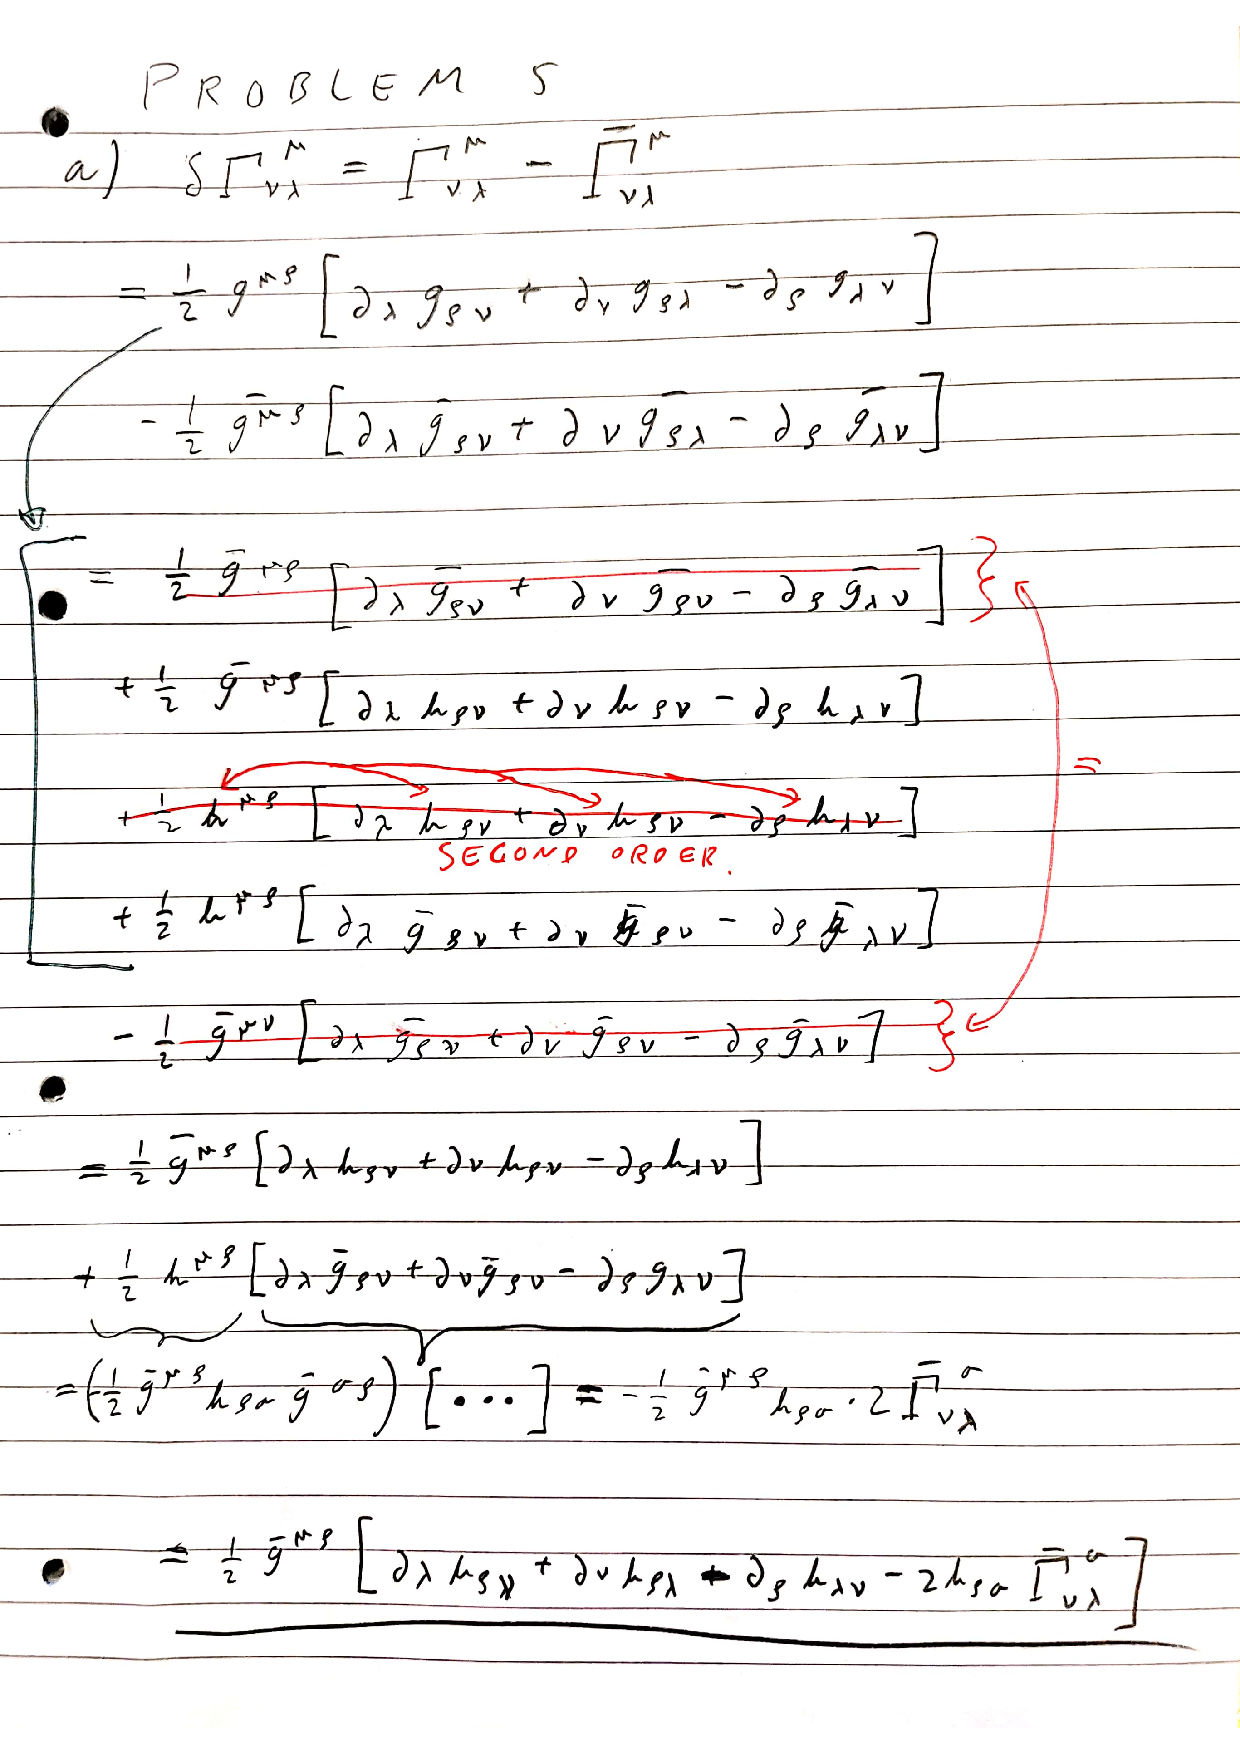
\includepdf[pages=1-]{problem5.pdf}


\end{document}